\documentclass[11pt,a4paper]{article}
\usepackage[margin=22mm]{geometry}
\usepackage{amsmath,amssymb,booktabs,tikz,enumitem,hyperref}
\usetikzlibrary{arrows.meta,positioning}
\setlength{\parindent}{0pt}\setlength{\parskip}{5pt}
\begin{document}
\begin{center}{\Large\bfseries Homework 1: Concise Answers}\end{center}
\section*{Intro1}
Rational action maximizes expected utility given the available information $I$:
\[
\boxed{a^*\in\arg\max_a\mathbb E[U\mid I,a]}.
\]
Rationality concerns the decision method; selfishness concerns the goal.
\[
U=U_{\rm self}\quad\text{(selfish)},\qquad
U=\alpha U_{\rm self}+\beta U_{\rm others}\quad\text{(may be altruistic)}.
\]
Example: compare price and quality, then choose the best expected value.
A rational choice may still have a bad outcome under uncertainty.

\section*{Intro2}
\textbf{Example: exhaustive game-tree search under a short time limit.}
For branching factor $b$ and search depth $d$,
\[
N_{\rm leaves}=b^d,\qquad
N_{\rm nodes}=\sum_{k=0}^d b^k=\frac{b^{d+1}-1}{b-1}\quad(b>1).
\]
Humans have limited memory and calculation speed. Computers can systematically enumerate and evaluate many moves; AI need not imitate human thinking.

\newpage
\section*{Intro3}
\textbf{LLM:} Codex; original discussion: October 8, 2026.\\
\textbf{Prompt:} Why did multilayer learning take years despite XOR needing only one extra hidden layer?

\begin{center}\begin{tabular}{cc|cc|c}\toprule
$x_1$&$x_2$&$z_1$ (OR)&$z_2$ (AND)&$y$ (XOR)\\\midrule
0&0&0&0&0\\0&1&1&0&1\\1&0&1&0&1\\1&1&1&1&0\\\bottomrule
\end{tabular}\end{center}
For a single linear threshold, XOR would require
\[
b<0,\quad w_1+b\ge0,\quad w_2+b\ge0,\quad w_1+w_2+b<0.
\]
But $w_1+w_2+b\ge-b>0$: contradiction. Thus XOR is not linearly separable.

Let $H(t)=\mathbf1[t\ge0]$. A nonlinear hidden layer solves XOR:
\begin{align*}
z_1&=H(x_1+x_2-0.5),&z_2&=H(x_1+x_2-1.5),\\
\boxed{y}&\boxed{=H(z_1-2z_2-0.5)}.&&
\end{align*}
\begin{center}
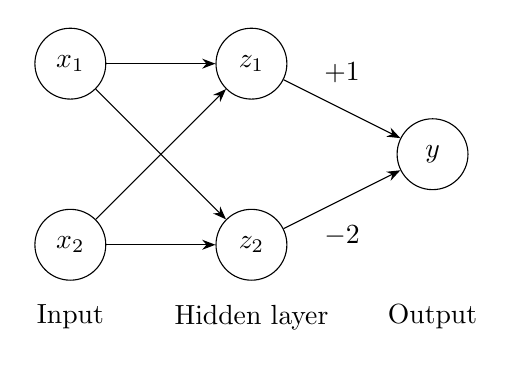
\begin{tikzpicture}[>=Stealth,every node/.style={draw,circle,minimum size=9mm},x=2.3cm,y=1.15cm]
\node (x1) at (0,1) {$x_1$};\node (x2) at (0,-1) {$x_2$};
\node (z1) at (1,1) {$z_1$};\node (z2) at (1,-1) {$z_2$};\node (y) at (2,0) {$y$};
\foreach \a in {x1,x2}\foreach \b in {z1,z2}\draw[->] (\a)--(\b);
\draw[->] (z1)--node[draw=none,above] {$+1$}(y);
\draw[->] (z2)--node[draw=none,below] {$-2$}(y);
\node[draw=none,rectangle] at (0,-1.8) {Input};
\node[draw=none,rectangle] at (1,-1.8) {Hidden layer};
\node[draw=none,rectangle] at (2,-1.8) {Output};
\end{tikzpicture}
\end{center}
\textbf{Difficulty: learning hidden weights, not drawing another layer.}
For differentiable activations, the chain rule gives credit assignment:
\[
\frac{\partial L}{\partial w^{(1)}}=
\frac{\partial L}{\partial y}\frac{\partial y}{\partial z}
\frac{\partial z}{\partial w^{(1)}},\qquad
w\leftarrow w-\eta\nabla_wL.
\]
Back-propagation + nonlinear differentiable units + gradient optimization make multilayer learning practical. The hard-threshold network above demonstrates representation, not differentiable training.

\begin{center}\small\begin{tabular}{c|l}\toprule
Year&Milestone\\\midrule
1969&Minsky--Papert: \emph{Perceptrons} [1]\\
1974&Werbos: backward differentiation for learning [3]\\
1986&Rumelhart--Hinton--Williams: back-propagation milestone [2]\\\bottomrule
\end{tabular}\end{center}
\[
\boxed{1986-1970=16\text{ years}}\qquad(1986-1969=17).
\]
The 1986 work popularized multilayer learning; it was not the first invention of hidden layers. ``Dead around 1970'' is a simplified description of declining interest.

{\footnotesize References: [1] Minsky and Papert, \emph{Perceptrons}, 1969.
[2] Rumelhart et al., \emph{Nature} 323, 533--536, 1986.
[3] Werbos, \emph{Beyond Regression}, Harvard thesis, 1974 (author's later account: \url{https://www.werbos.com/AD2004.pdf}).}
\end{document}
